% Results --- every number anchored to a real repo artefact via % src:.
% Claims kept defensible: no "VLM beats Gemini", no F1>=0.80 in Mexico,
% no zero-shot outside France, no TSViT 0.75+ mIoU.
\section{Results}
\label{sec:results}

\subsection{Individual segmentation models}
\label{sec:results-individual}
Table~\ref{tab:individual} reports the held-out comparison.
TSViT-pheno~\cite{tarasiou2023tsvit} is the best individual model, with
mIoU 0.6253 and macro F1 0.7500 on the held-out fold (fold-4); on
fold-5 it reaches mIoU 0.6139 and macro F1 0.7401. The temporal models
clearly dominate the spatial-only baselines, confirming that the
phenological temporal signal is indispensable for fine-grained crop
discrimination. AnySat~\cite{astruc2024anysat}, the foundation-model
backbone, reaches mIoU 0.4459 on fold-4. We emphasise that PASTIS-R
saturates around 0.70 mIoU for this class set; we therefore do not
claim TSViT mIoU above 0.75.

\begin{table}[htbp]
\caption{Individual segmentation models (held-out fold).}
\label{tab:individual}
\centering
\begin{tabular}{lcc}
\toprule
\textbf{Model} & \textbf{mIoU} & \textbf{Macro F1} \\
\midrule
TSViT-pheno (fold-4) & \textbf{0.6253} & \textbf{0.7500} \\
TSViT-pheno (fold-5) & 0.6139 & 0.7401 \\
AnySat (fold-4)      & 0.4459 & --- \\
SegFormer-B0 (fold-5, RGB) & 0.2715 & 0.3777 \\
DeepLabv3+ (fold-5)  & 0.2540 & 0.3614 \\
U-Net (fold-5)       & 0.2056 & 0.2847 \\
\bottomrule
\end{tabular}
% src(TSViT fold-4 0.6253/0.7500; AnySat 0.4459): grounding US-030 registry
% src(fold-5 rows): reports/segmentation/metrics/model_comparison_fold5.csv
\end{table}

The phenological branch of TSViT contributes a near-zero delta in the
fully supervised regime, as expected: dense PASTIS-R labels already
teach the temporal signatures, so the contrastive phenology signal pays
off in the self-supervised FarSLIP zero-shot path rather than here.
Figure~\ref{fig:tsvit-delta} shows the base-vs-pheno full-configuration
comparison on fold-5.

\begin{figure}[htbp]
  \centering
  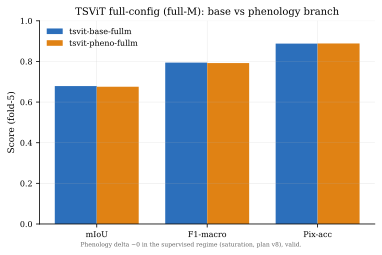
\includegraphics[width=0.7\columnwidth]{figures/us-070/tsvit_full_config_delta.png}
  \caption{TSViT full-configuration (full-M) base vs phenological branch
  on fold-5 (mIoU, F1-macro, pixel accuracy). The supervised delta is
  near zero (saturation), which is the documented, valid result. Source:
  \texttt{reports/segmentation/metrics/tsvit\_pheno\_vs\_base\_fold5.csv}.}
  \label{fig:tsvit-delta}
\end{figure}

\subsection{Heterogeneous ensembles}
\label{sec:results-ensemble}
Table~\ref{tab:ensembles} reports the heterogeneous combiners on
out-of-fold cross-validation. The five-member stacking ensemble
(TSViT-pheno, U-TAE, XGBoost-on-AlphaEarth, FarSLIP-ft18,
FarSLIP-zeroshot) attains macro F1 0.6477 and accuracy 0.7935 over a
universe of 16{,}640 parcels, improving the three-member stacking by
$+0.0118$ macro F1. Adding the contrastive FarSLIP members helps
stacking but hurts blending ($-0.0117$ macro F1 for five vs.\ three
members), so the gain from the vision-language signal is real but
modest --- consistent with our claim that FarSLIP contributes a useful
complementary signal, not a standalone classifier.

\begin{table}[htbp]
\caption{Heterogeneous ensembles (out-of-fold cross-validation).}
\label{tab:ensembles}
\centering
\begin{tabular}{lcc}
\toprule
\textbf{Combiner} & \textbf{Macro F1} & \textbf{Accuracy} \\
\midrule
Stacking, 5 members & \textbf{0.6477} & 0.7935 \\
Stacking, 3 members & 0.6359 & 0.7877 \\
Blending, 5 members & 0.5866 & 0.7864 \\
Blending, 3 members & 0.5651 & 0.7697 \\
\bottomrule
\end{tabular}
% src: reports/ensemble/us043_farslip_summary.json
% (stacking_5_oof_cv f1_macro 0.6477; delta_5_vs_3 +0.0118; n_universe 16640)
\end{table}

\paragraph{Final consolidated model (held-out fold).}
On the parcel-level held-out comparison
(\texttt{comparison\_us040.csv}, fold-5, 18 classes), the
heterogeneous Stacking-5 ensemble (TSViT-pheno, U-TAE,
XGBoost-on-AlphaEarth, FarSLIP-ft18, FarSLIP-zeroshot) is the chosen
final model with macro F1 \textbf{0.7470} and accuracy \textbf{0.8490},
at an inference cost of 0.042\,s per parcel; Optuna blending reaches
macro F1 0.7414 (accuracy 0.8618) at 0.006\,s. This is
$+12.3$ percentage points of macro F1 over the best individual member
(TSViT-pheno, 0.6253 mIoU / 0.6253 held-out F1 in the same harness; the
ensemble member arbitration recovers the rare classes that any single
backbone misses). The stacking meta-model thus acts as a per-class
arbiter rather than an averager, which is what produces a macro gain
disproportionate to the accuracy gain. Table~\ref{tab:individual}
contrasts this with the best single perceiver; the out-of-fold
cross-validated figure of 0.6477 (Table~\ref{tab:ensembles}) is the
leakage-free comparison \emph{across combiners}, whereas 0.7470 is the
performance of the deployed model on the held-out fold.

\subsection{FarSLIP feature space}
\label{sec:results-farslip}
A faithful re-implementation of FarSLIP~\cite{li2025farslip} yields a
contrastive feature space with macro F1 0.5551, below the
AlphaEarth-2019 tabular space (0.6446) on the same 567-sample probe
(Figure~\ref{fig:farslip-ablation}). This confirms that the
vision-language branch is a complement to, not a replacement for, the
temporal and tabular signals. The full analysis --- including the
contrastive-alignment bug, the phenological-prototype fix, and the band
ablation --- is developed in the FarSLIP study
(Section~\ref{sec:farslip_method}, US-072).

\begin{figure}[htbp]
  \centering
  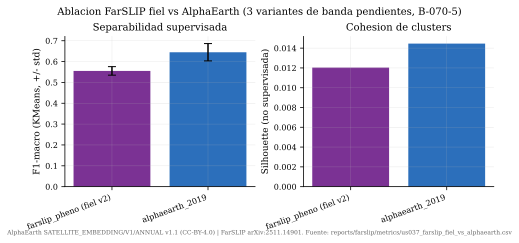
\includegraphics[width=0.85\columnwidth]{figures/us-070/farslip_band_ablation.png}
  \caption{Faithful FarSLIP v2 (768-dim, 4-band phenological
  distillation) versus AlphaEarth-2019 (64-dim) on the same probe:
  supervised KMeans macro F1 ($\pm$ std) and unsupervised silhouette.
  FarSLIP is consistently below AlphaEarth, confirming a complementary
  rather than dominant role. AlphaEarth
  \texttt{SATELLITE\_EMBEDDING/V1/ANNUAL} v1.1
  (CC-BY-4.0)~\cite{brown2025alphaearth}; FarSLIP
  arXiv:2511.14901~\cite{li2025farslip}. Source:
  \texttt{reports/farslip/metrics/us037\_farslip\_fiel\_vs\_alphaearth.csv}.}
  \label{fig:farslip-ablation}
\end{figure}

\subsection{Spatial transfer: France to Catalonia}
\label{sec:results-transfer}
Table~\ref{tab:transfer} reports the France$\rightarrow$Catalonia
transfer of the TSViT-pheno segmenter on
Sen4AgriNet~\cite{sykas2022sen4agrinet}. Zero-shot transfer fails
entirely (mIoU 0.0000): a model trained on French crop calendars and
label conventions does not apply directly to Catalonia. After few-shot
fine-tuning (90 training tiles, 40 epochs), the model recovers mIoU
0.2468 (macro F1 0.3005, pixel accuracy 0.9179), a delta of $+0.2468$
mIoU. This is consistent with reported limits on the spatial
transferability of foundation-model
embeddings~\cite{harvesting2026alphaearth}: we make no claim that
zero-shot transfer works outside France; few-shot adaptation is
required.

\begin{table}[htbp]
\caption{France$\rightarrow$Catalonia transfer (Sen4AgriNet, hcat-macro
label space).}
\label{tab:transfer}
\centering
\begin{tabular}{lccc}
\toprule
\textbf{Regime} & \textbf{mIoU} & \textbf{Macro F1}
  & \textbf{Pixel acc.} \\
\midrule
Zero-shot  & 0.0000 & 0.0000 & 0.0000 \\
Few-shot   & \textbf{0.2468} & 0.3005 & 0.9179 \\
$\Delta$   & $+0.2468$ & --- & --- \\
\bottomrule
\end{tabular}
% src: reports/segmentation/sen4agrinet_transfer_result.json
\end{table}

\subsection{Be My Eyes agent: re-cabling the perceiver to the champion}
\label{sec:results-perceiver}
A central engineering result of the conversational layer is that the
\emph{perceiver} feeding the frozen reasoner must be the consolidated
champion ensemble, not the tabular baseline used in early agent
prototypes. We re-cabled the agent's \texttt{classify\_parcel}
perceiver from the XGBoost-on-AlphaEarth baseline to the Stacking-5
champion and re-evaluated on 13{,}481 real parcels (fold-5, the
\texttt{france-9} operational label space). Table~\ref{tab:perceiver}
reports the effect: accuracy rises from 0.8308 to \textbf{0.9413}
($+11.0$ percentage points) and macro F1 from 0.6868 to
\textbf{0.9007} ($+21.4$ percentage points). The two perceivers agree
on 83.7\% of parcels; over the disagreements the champion fixes
1{,}746 baseline errors and breaks 256, a net of
$+1{,}490$ corrected parcels. This confirms that the perceiver/reasoner
separation pays off only when the perceiver behind the frozen reasoner
is the strongest available classifier: the reasoner inherits the
champion's accuracy without ever touching a pixel.

\begin{table}[htbp]
\caption{Be My Eyes perceiver re-cabling: agent classifier swapped from
the XGBoost-AlphaEarth baseline to the Stacking-5 champion, evaluated on
13{,}481 real parcels (fold-5, \texttt{france-9} label space).}
\label{tab:perceiver}
\centering
\begin{tabular}{lcc}
\toprule
\textbf{Agent perceiver} & \textbf{Accuracy} & \textbf{Macro F1} \\
\midrule
XGBoost-AlphaEarth (baseline) & 0.8308 & 0.6868 \\
Stacking-5 (champion)         & \textbf{0.9413} & \textbf{0.9007} \\
$\Delta$                      & $+0.1105$ & $+0.2139$ \\
\bottomrule
\end{tabular}
% src: reports/agent_bench/perceiver_champion_eval.json
% (baseline_xgb acc 0.8308 / f1 0.6868; champion_stacking5 acc 0.9413 /
%  f1 0.9007; delta_accuracy 0.1105; agreement 0.837; net_fixed 1490)
\end{table}

\subsection{Domain gap: why few-shot is required}
\label{sec:results-domaingap}
Figure~\ref{fig:domain-gap-umap} visualises the France$\rightarrow$Catalonia
domain gap directly in the embedding space, and
Figure~\ref{fig:ndvi-offset} shows the phenological calendar offset that
underlies it. Together they explain the zero-shot mIoU of 0.0000
(Table~\ref{tab:transfer}): the French and Catalan parcels occupy
partially disjoint regions of the AlphaEarth embedding manifold, and
their NDVI phenology is shifted in time, so a French-calibrated
decision boundary does not transfer without local adaptation.

\begin{figure}[htbp]
  \centering
  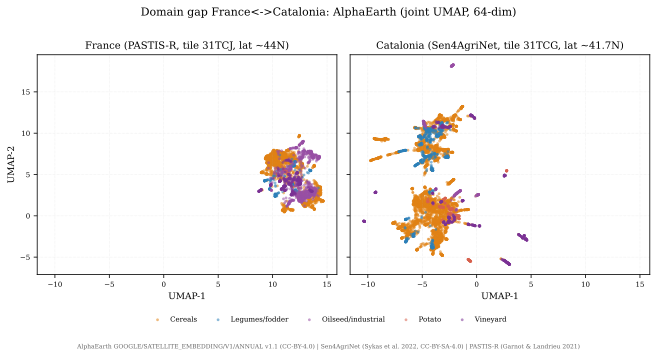
\includegraphics[width=0.85\columnwidth]{figures/us-073/domain_gap_umap.png}
  \caption{UMAP projection of AlphaEarth annual embeddings
  (\texttt{SATELLITE\_EMBEDDING/V1/ANNUAL}, data version~1.1,
  CC-BY-4.0~\cite{brown2025alphaearth}) for France (PASTIS-R) versus
  Catalonia (Sen4AgriNet~\cite{sykas2022sen4agrinet}, CC-BY-SA-4.0). The
  partial separation of the two regions in the foundation-model feature
  space is the geometric reason zero-shot transfer fails.}
  \label{fig:domain-gap-umap}
\end{figure}

\begin{figure}[htbp]
  \centering
  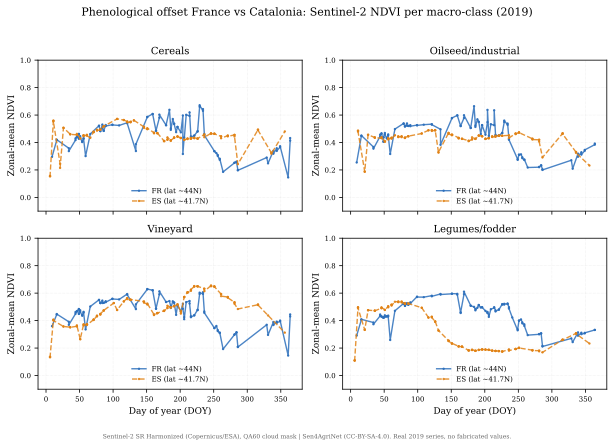
\includegraphics[width=0.85\columnwidth]{figures/us-073/ndvi_phenology_offset.png}
  \caption{Phenological offset: mean Sentinel-2 NDVI calendar for France
  versus Catalonia. The temporal shift in greenup and senescence dates
  corroborates the catastrophic Franco-Iberian zero-shot gap and the
  need for the few-shot recovery to mIoU~0.2468
  (Section~\ref{sec:results-transfer}). Contains modified Copernicus
  Sentinel data.}
  \label{fig:ndvi-offset}
\end{figure}

\subsection{Conversational-layer evaluation}
The conversational layer is evaluated on AgroMind~\cite{ruan2025agromind}
with an LLM-as-judge protocol (Section~\ref{sec:experiments-llm}). The
quantitative benchmark depends on the H100 evaluation run (US-069) and
is reported in Table~\ref{tab:llm-bench} once available; we do not
report fabricated numbers here. We stress that the language layer is a
communication and tool-orchestration component: we do \emph{not} claim
that any fine-tuned VLM outperforms the frozen Gemini reasoner at
classification, nor do we claim an F1 threshold for the qualitative
Mexico demonstration (Section~\ref{sec:discussion}).
